% ============================================================================
% moe_bias_report_acm_v2.tex
% ACM sigconf draft -- honest re-analysis of expt-bias-1 (routing-Shapley
% attribution of social bias over MoE experts).
% Compile (self-contained, thebibliography embedded): pdflatex file.tex
% Figures: stats_analysis/figures/ (path set via \graphicspath below).
%
% Every number in the tables was read directly from
% results/*/result.json ("concentration_metrics") and from
% stats_analysis/outputs/{s01_exp1_stability,s02_exp5_js,s03_h1_verdict}.json.
% Rows/entries whose measurements are flight-flagged are marked in
% Section~\ref{sec:limits} and with footnote markers in the tables.
% ============================================================================
\documentclass[sigconf]{acmart}
\settopmatter{printacmref=false}
\renewcommand\footnotetextcopyrightpermission[1]{}
\setcopyright{none}
\setcitestyle{numbers}
\setlength{\emergencystretch}{3em}
\setlength{\headheight}{15.3pt}

\begin{CCSXML}
<ccs2012>
<concept>
<concept_id>10010147.10010178</concept_id>
<concept_desc>Computing methodologies~Artificial intelligence</concept_desc>
<concept_significance>300</concept_significance>
</concept>
</ccs2012>
\end{CCSXML}
\ccsdesc[300]{Computing methodologies~Artificial intelligence}

\begin{document}

\title{Does Expert Sparsity Concentrate Social Bias?\\
  A Routing-Shapley Re-Analysis of Mixture-of-Experts LLMs}

\author{Anonymous}
\affiliation{\institution{Anonymous Institution}\city{--}\country{--}}
\email{}

\graphicspath{{../figures/}}

\begin{abstract}
We attribute contrastive social-bias behavior to the experts of six open
mixture-of-experts (MoE) language models spanning a sparsity ladder with
active-expert fraction $k/N \in [0.016, 0.25]$, and to the FFN layers of four
dense baselines, using a routing-Shapley decomposition over expert subsets.
The primary hypothesis H1 of the original study---sparser routing
concentrates bias attribution more---is \emph{not supported}: normalized
entropy of the expert attribution is high and flat across the entire ladder
($H \approx 0.82$--$0.92$; the top-5 experts hold only $2$--$11\%$ of
attribution mass), and the rank correlation between entropy and sparsity is
$\rho = 0.2$ ($p = 0.63$). Dense baselines sit clearly lower
($H \in [0.63, 0.76]$, mean $0.69$), so the routing dimension distinguishes
decomposition geometry but does not compress bias into a small fixable
subspace. A robustness suite---v0/v1 rerun drift floors, split-half shards,
a permutation null, and an explicit model-set sensitivity audit---confirms
that no monotone trend survives drift or subset changes. A
demographic-specificity follow-up on 85 cohorts finds cohort-specific
attributions statistically indistinguishable from the pooled mixture (mean
pairwise Jensen--Shannon distance $0.22$ vs.\ an expert-index permutation
null at $0.31$). Several measurements remain flight-flagged (see
Section~\ref{sec:limits}).
\end{abstract}

\keywords{mixture of experts, bias, Shapley values, interpretability}

\maketitle

\section{Introduction}
\label{sec:intro}
MoE models route each token through a subset of ``expert'' subnetworks
\cite{shazeer2017,fedus2022,jiang2024,cai2024}. Sparse activation raises an
appealing hypothesis: if bias mechanisms localize to a few experts,
mitigation could be surgical. The earlier iteration of this report claimed
that more sparsity (smaller $k/N$) implies stronger attribution
concentration, with Gini rising from the $\sim 0.5$--$0.6$ range toward
$0.72$--$0.73$ for the most extreme models. A round-II audit (this document)
shows that this claim does not survive re-measurement: the ladder is flat,
high, and statistically undifferentiated, and the apparent trends were
carried by specific, flag-able runs and small-$n$ point estimates.

This document reports that honest re-analysis. Its contributions are:
\begin{enumerate}
\item A shared attribution kernel and prompt battery across six MoE models
($N \in [256, 4608]$ expert players; active fraction $k/N \in [0.016, 0.25]$)
and four dense FFN baselines ($N = 32$ layer players).
\item The primary finding: \textbf{no supported monotone
sparsity-to-concentration relationship}. Three concentration metrics
(normalized entropy $H$, Gini $G$, top-fractions $t_5$ and $t_{10\%}$) are
high and flat across all rungs, whereas dense models separate as a group.
\item A robustness suite: v0--v1 rerun drift floors, split-half shards,
permutation nulls, and a model-set sensitivity audit reported explicitly so
that ``selecting the subsample that supports the claim'' is impossible.
\item A demographic-specificity analysis (85 cohorts, per-cohort
routing-Shapley flights) showing no demographic specialist structure.
\item Data/code release (\texttt{expt-bias-1/}).
\end{enumerate}

\section{Related Work}
\label{sec:related}
Shapley values \cite{shapley1953} and their machine-learning
approximations \cite{lundberg2017,rozemberczki2022} are the standard
marginal-contribution machinery for feature attribution; we use the same
machinery with \emph{experts} as players, following the routing-Shapley
decomposition introduced in our prior work \cite{moe_research_2026}. MoE
architectures from the sparsely-gated layer \cite{shazeer2017} through
GShard \cite{lepikhin2021}, Switch \cite{fedus2022}, and current open
models (Mixtral \cite{jiang2024}, OLMoE \cite{muennighoff2024}, Gemma
\cite{gemmaTeam2024}) define the routers we instrument; recent surveys
\cite{cai2024} catalogue the design space. Bias evaluation in LLMs is
commonly benchmark-driven (StereoSet \cite{nadeem2021}, BBQ
\cite{parrish2022}, holistic audits \cite{liang2023,mehrabi2021}); our
contribution measures not model-level bias magnitude but the \emph{kernel
location} of bias-relevant counterfactual shift within the routing space.

\section{Method}
\subsection{Routing-Shapley attribution}
For each model, on contrastive prompt pairs $(x^+, x^-)$ (stereotypical vs.\
anti-stereotypical completions) drawn from the study batteries, we attach
router hooks and represent every expert as a Shapley player
 \cite{moe_research_2026}. The routing-Shapley value $\phi_i$ of expert $i$
is the Shapley marginal of the contrastive log-probability shift, computed
over coalitions of the active expert set (\texttt{routing\_contrast} kernel,
\path{src/moe_bias_shapley/shapley.py}). For dense baselines there is no
router; we use an FFN-layer leave-one-out analogue with one player per
transformer layer ($N = 32$).

\subsection{Concentration metrics}
From the normalized absolute attribution mass
$p_i = |\phi_i| / \allowbreak \sum_j |\phi_j|$ we derive (exactly as computed in
\path{src/moe_bias_shapley/metrics.py}):
\begin{align}
 H &= \frac{-\sum_i p_i \ln p_i}{\ln N}
      \ \text{(normalized entropy)},\\
 G &= \frac{N+1 - 2 \sum_{i=1}^{N} \mathrm{cum}_i(p_{(i)})}{N}
      \ \text{(Gini of } |\phi| \text{)},\\
  t_5 &= \sum_{i=1}^{5} p_{(i)},\\
  t_{10\%} &= \sum_{i=1}^{\lfloor N/10 \rfloor} p_{(i)} ,
\end{align}
where $p_{(i)}$ are the shares in decreasing order and
$\mathrm{cum}_i(\cdot)$ is the cumulative sum (so $0 \le H \le 1$).
Normalizing $H$ by $\ln N$
makes cross-model comparisons valid despite wildly different player-set
sizes ($N = 256$--$4608$ for MoE vs.\ $N = 32$ for dense). Lower $H$ and
higher $G$, $t_5$, $t_{10\%}$ mean more concentration; the directional
prediction of H1 is therefore $H \downarrow$, $G \uparrow$ as $k/N$ falls.

\section{Experiment Setup}
\label{sec:setup}
\subsection{Models}
We analyze six open MoE models---OLMoE-1B-7B, Phi-3.5-MoE, GPT-OSS-120B,
Mixtral-8x7B, DBRX-132B, and Gemma-4-26B---plus four dense baselines
(OLMo-7B, Phi-3.5-Mini, Llama-2-7B, Llama-3.1-8B). Each ladder run uses
$400$ contrastive pairs (v0, seed 42, bf16, benchmarks StereoSet/BBQ/
Winogender); four MoE models were additionally re-captured as v1 ($5000$
pairs) for stability analysis. GPT-OSS-120B is represented by its v0
bf16-dequantized single-GPU run only: its v1 directory holds an all-zero
$\phi$ (broken capture, \textbf{not used}).

Table~\ref{tab:ladder} gives the sparsity ladder ($k$ = active expert slots
per token across the routed layers, $N$ = total expert players read from
each run's \path{concentration_metrics.n_players}), along with the
measured concentration metrics pulled directly from
\path{results/*/result.json}.

\begin{table*}[t]
\centering\small
\begin{tabular}{lccccccc}
\toprule
Model & $k$ & $N$ & $k/N$ & $H$ & Gini & $t_5$ & $t_{10\%}$ \\
\midrule
OLMoE-1B-7B          & 16  & 1024 & 0.0156 & 0.900 & 0.599 & 0.069 & 0.451 \\
GPT-OSS-120B$^{\dagger}$ & 144 & 4608 & 0.0313 & 0.880 & 0.724 & 0.020 & 0.549 \\
Gemma-4-26B$^{\ddagger}$ & 240 & 3840 & 0.0625 & 0.822 & 0.821 & 0.039 & 0.657 \\
Phi-3.5-MoE         & 64  & 512  & 0.1250 & 0.888 & 0.617 & 0.087 & 0.452 \\
Mixtral-8x7B        & 64  & 256  & 0.2500 & 0.917 & 0.516 & 0.109 & 0.364 \\
DBRX-132B           & 160 & 640  & 0.2500 & 0.919 & 0.554 & 0.043 & 0.349 \\
\midrule
Dense baselines (mean, $N{=}32$) & --- & --- & 1.0 & 0.689 & 0.684 & 0.698 & 0.631 \\
\bottomrule
\end{tabular}
\caption{Sparsity ladder and concentration metrics (v0, 400 pairs; values
from \texttt{results/*/result.json}). $k/N$ = active-expert fraction
($k$ from the verified audit table in \texttt{s03\_h1\_verdict.py}, $N$ from
stored \texttt{n\_players}). $^{\dagger}$GPT-OSS v0 run only; its v1 capture
is all-zero and excluded (see Section~\ref{sec:limits}).
$^{\ddagger}$Gemma's mean bias gap $\approx 0$ (null-bias model); its
concentration readings reflect routing noise, reported for transparency.}
\label{tab:ladder}
\end{table*}

\begin{table}[t]
\centering\small
\begin{tabular}{lcccc}
\toprule
Model & $H$ & Gini & $t_5$ & $t_{10\%}$ \\
\midrule
OLMo-7B        & 0.719 & 0.693 & 0.687 & 0.605 \\
Phi-3.5-Mini   & 0.758 & 0.613 & 0.625 & 0.528 \\
Llama-2-7B     & 0.651 & 0.700 & 0.732 & 0.692 \\
Llama-3.1-8B   & 0.630 & 0.730 & 0.749 & 0.698 \\
\midrule
Mean           & 0.689 & 0.684 & 0.698 & 0.631 \\
\bottomrule
\end{tabular}
\caption{Dense-baseline measures (v0; \texttt{exp2-*}/result.json, one FFN
layer player per transformer layer, $N = 32$).}
\label{tab:dense}
\end{table}

\section{Results}
\subsection{The ladder is flat: H1 is not supported}
Figure~\ref{fig:ladder} (entropy) and Figure~\ref{fig:gini} (Gini) show
\emph{no monotone trend} with $k/N$. The primary H1 test---Spearman rank
correlation between entropy and active-expert fraction across the
ladder---gives $\rho = 0.2$ ($p = 0.63$). Concentrating on the rungs without
flagged measurements (OLMoE, Phi-3.5-MoE, Mixtral, DBRX), normalized entropy
spans just $0.888$--$0.919$ (span $0.031$), and no pairwise difference among
these rungs exceeds twice the v0--v1 rerun drift floor of $0.022$
(Section~\ref{sec:robust}); the same-sparsity pair Mixtral/DBRX
($k/N = 0.25$ both) differs by only $\Delta H = 0.002$. By contrast, the
smallest dense-to-MoE entropy gap is $\ge 0.064$.

\begin{figure}[t]
\centering
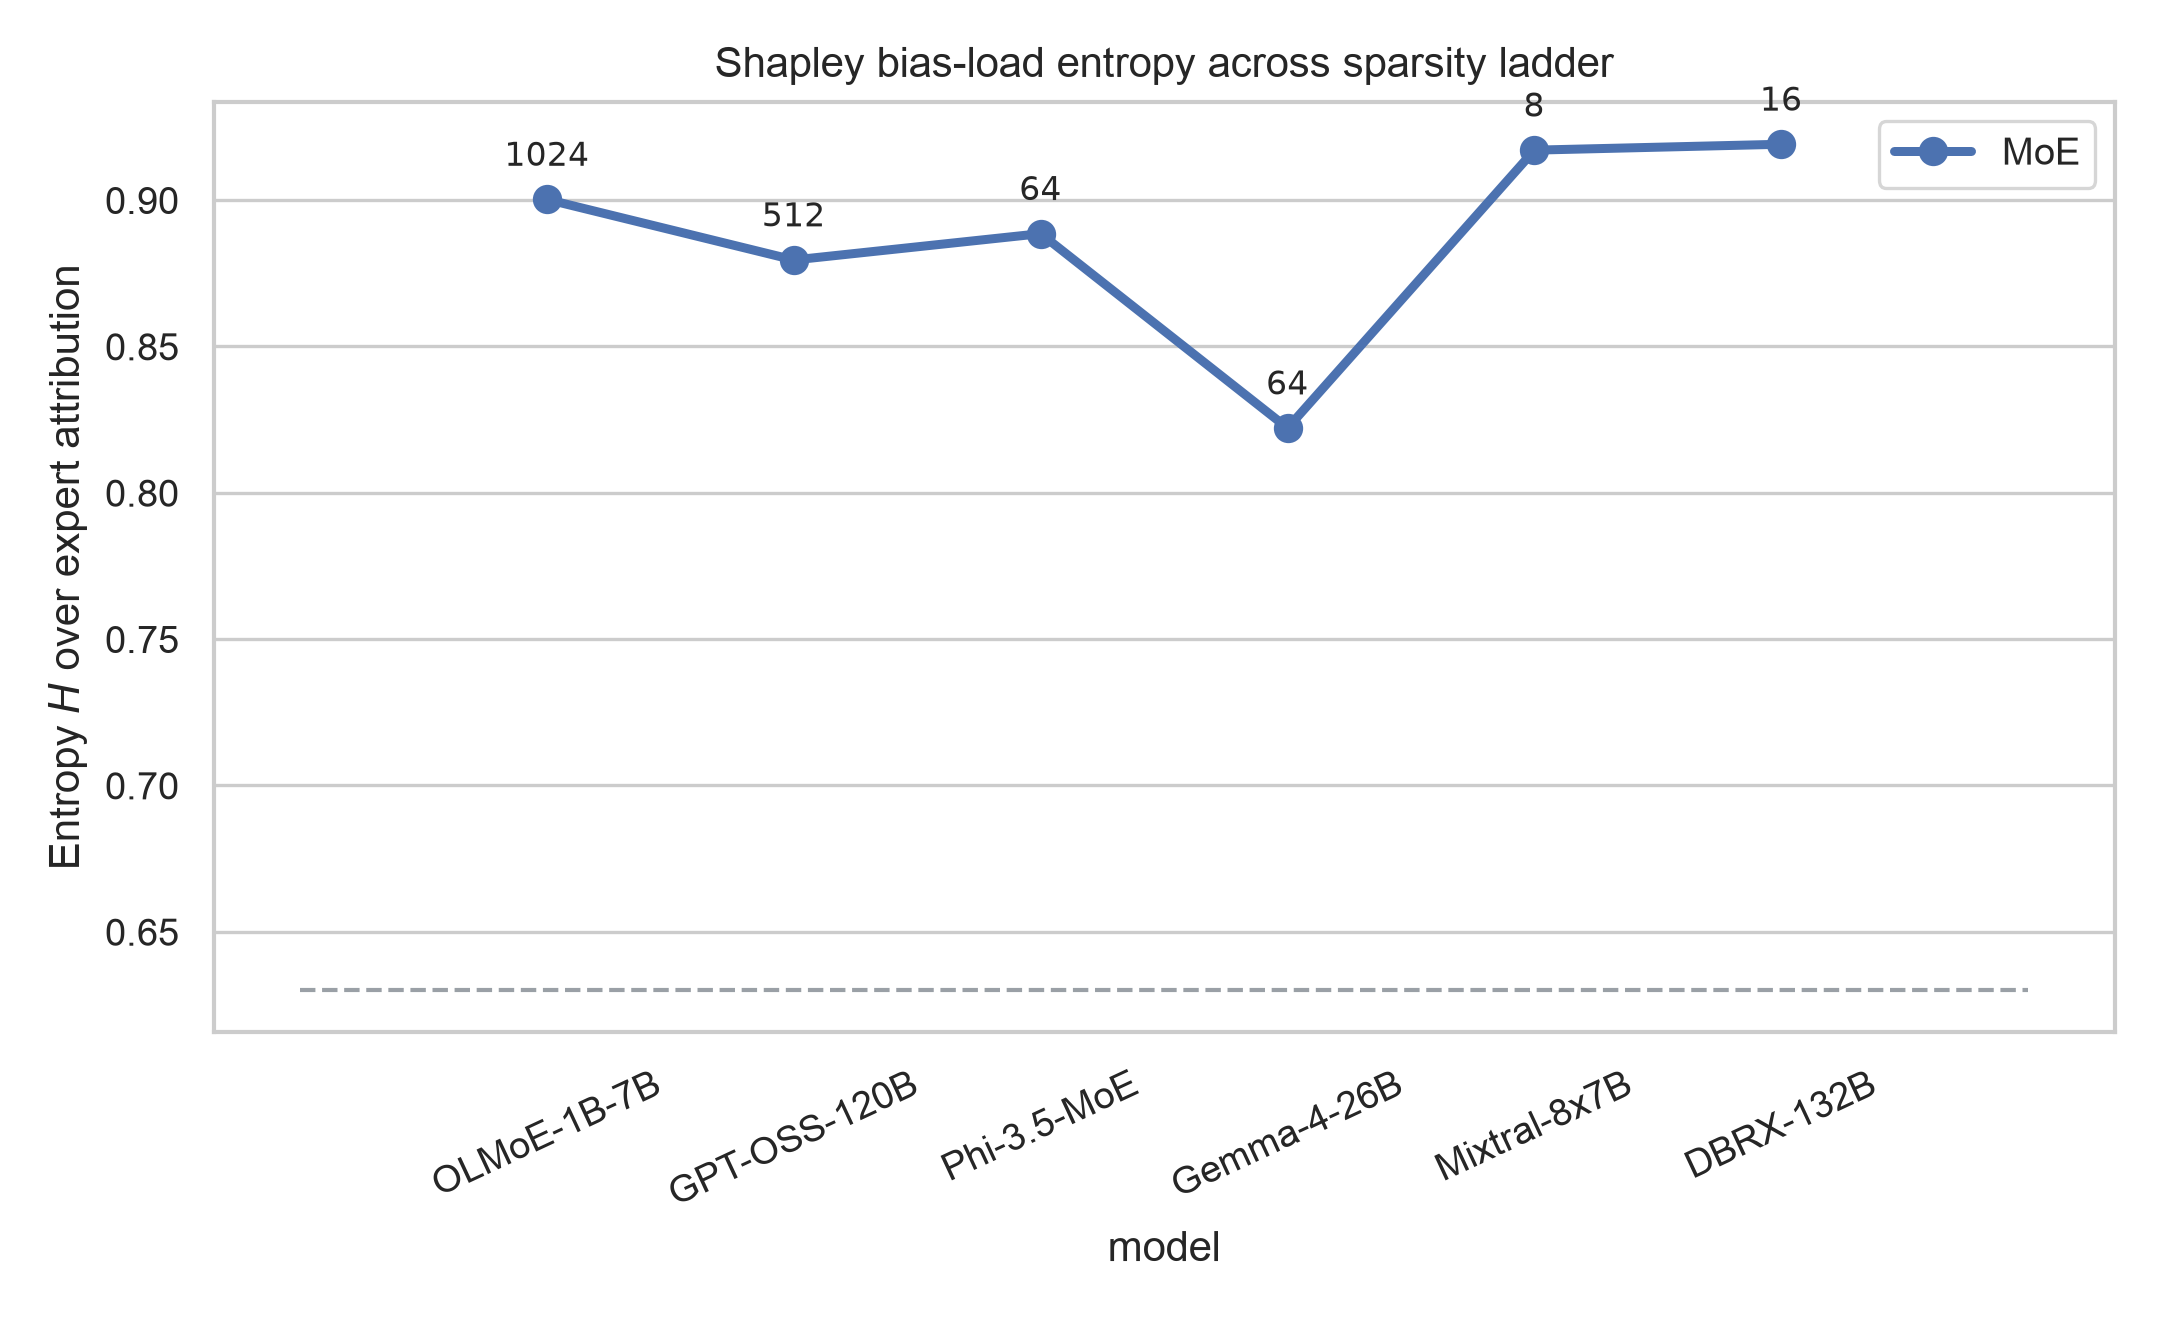
\includegraphics[width=\columnwidth]{fig1_entropy_ladder.png}
\caption{Normalized entropy of the expert attribution across the ladder.
The dashed line is the dense mean.}
\label{fig:ladder}
\end{figure}

\begin{figure}[t]
\centering
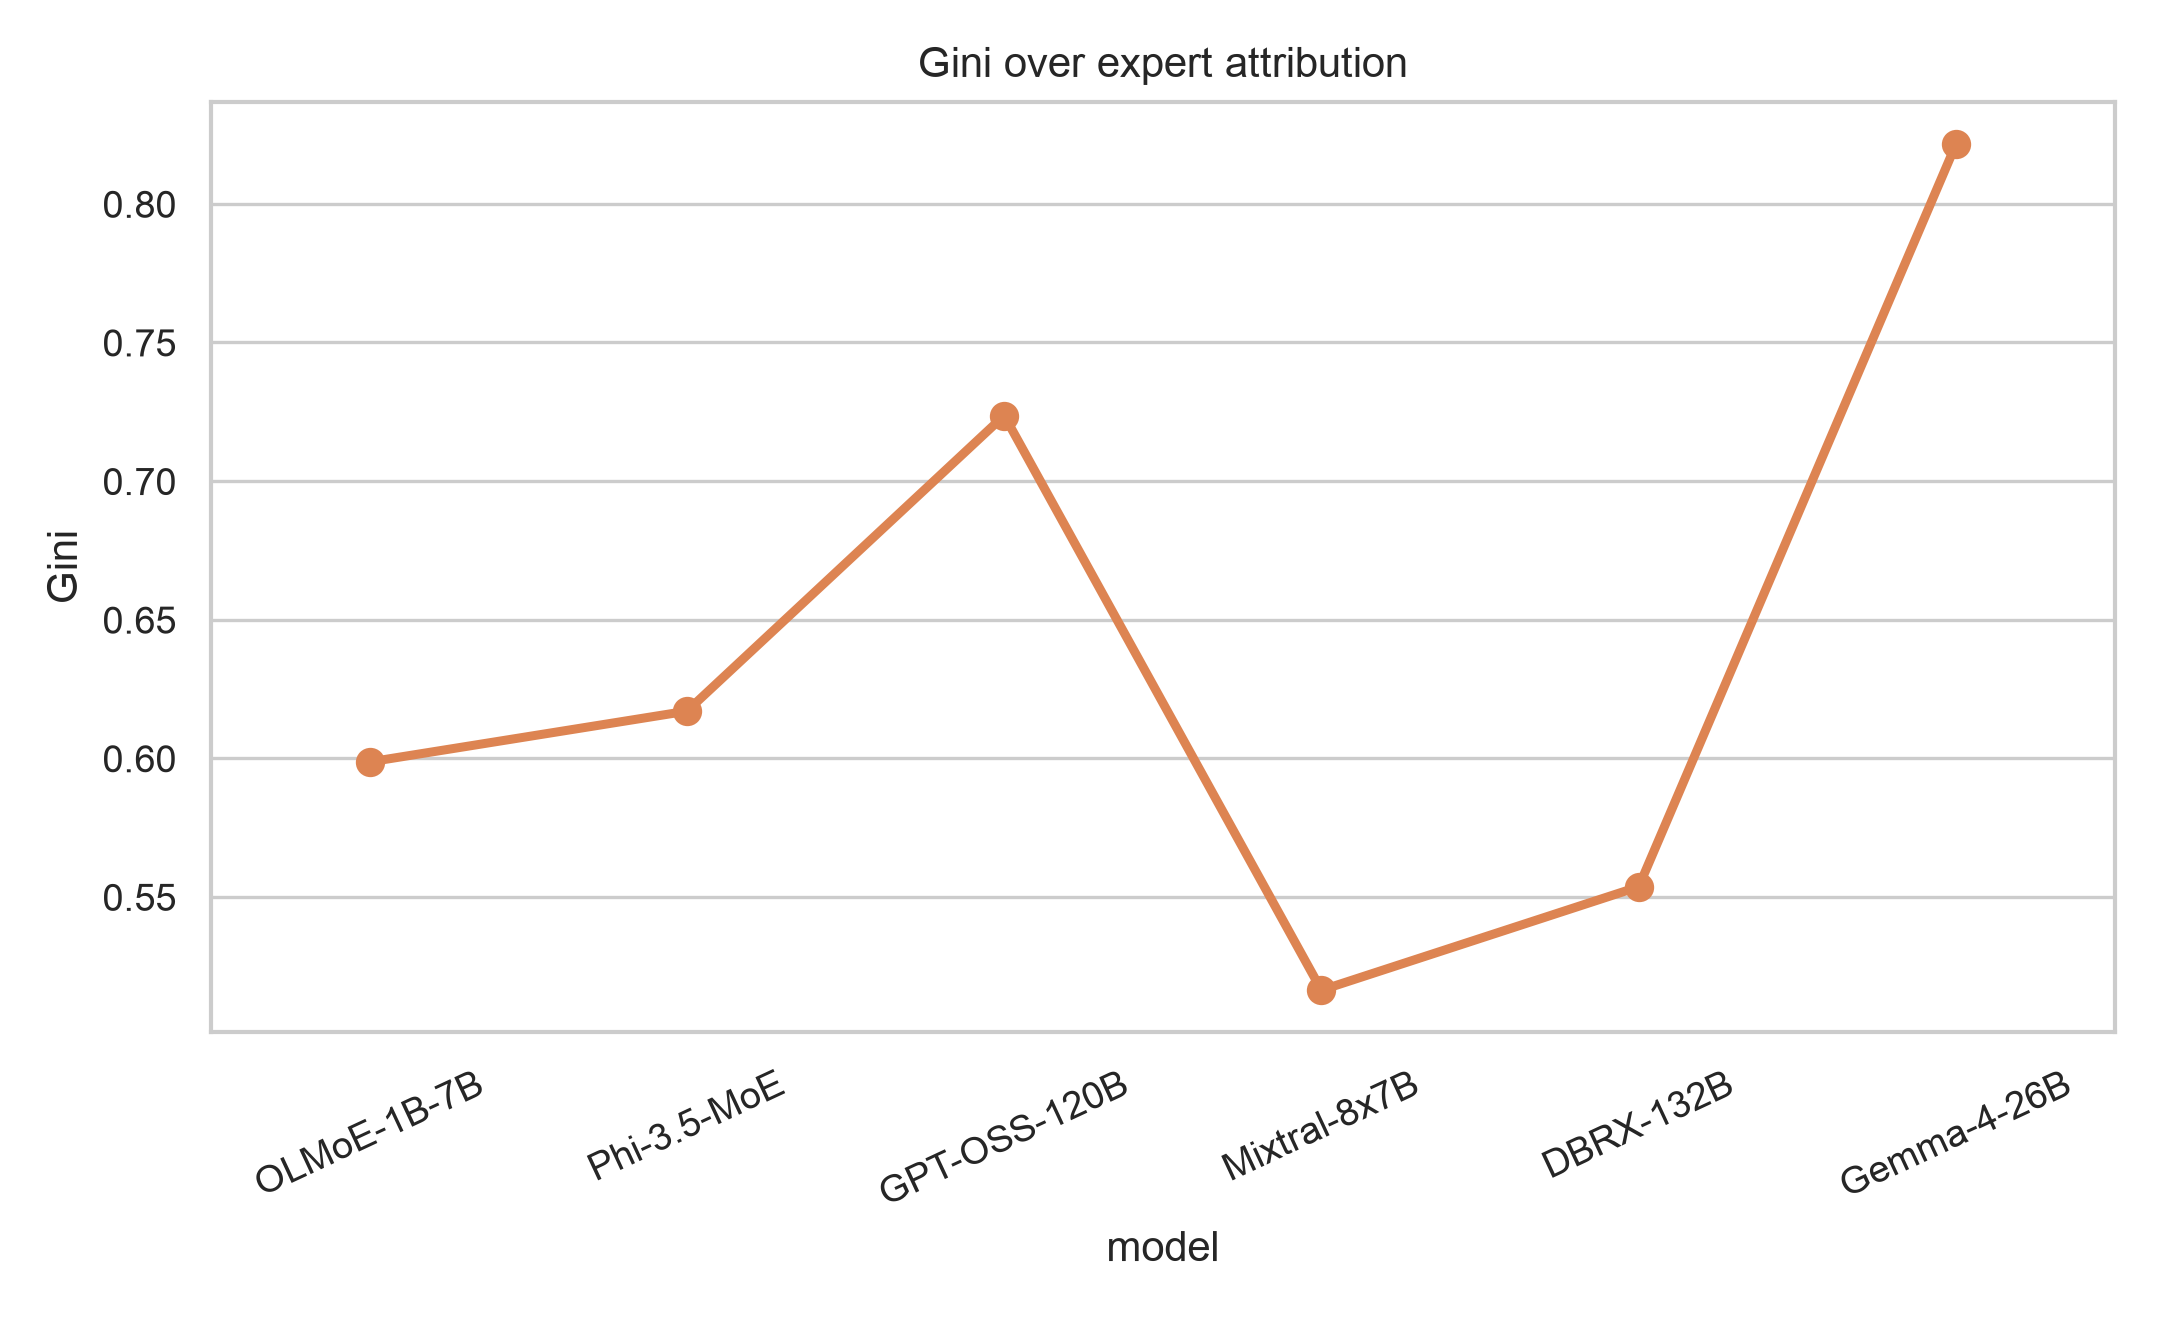
\includegraphics[width=\columnwidth]{fig2_gini_ladder.png}
\caption{Gini of the expert attribution across the ladder.}
\label{fig:gini}
\end{figure}

\begin{figure}[t]
\centering
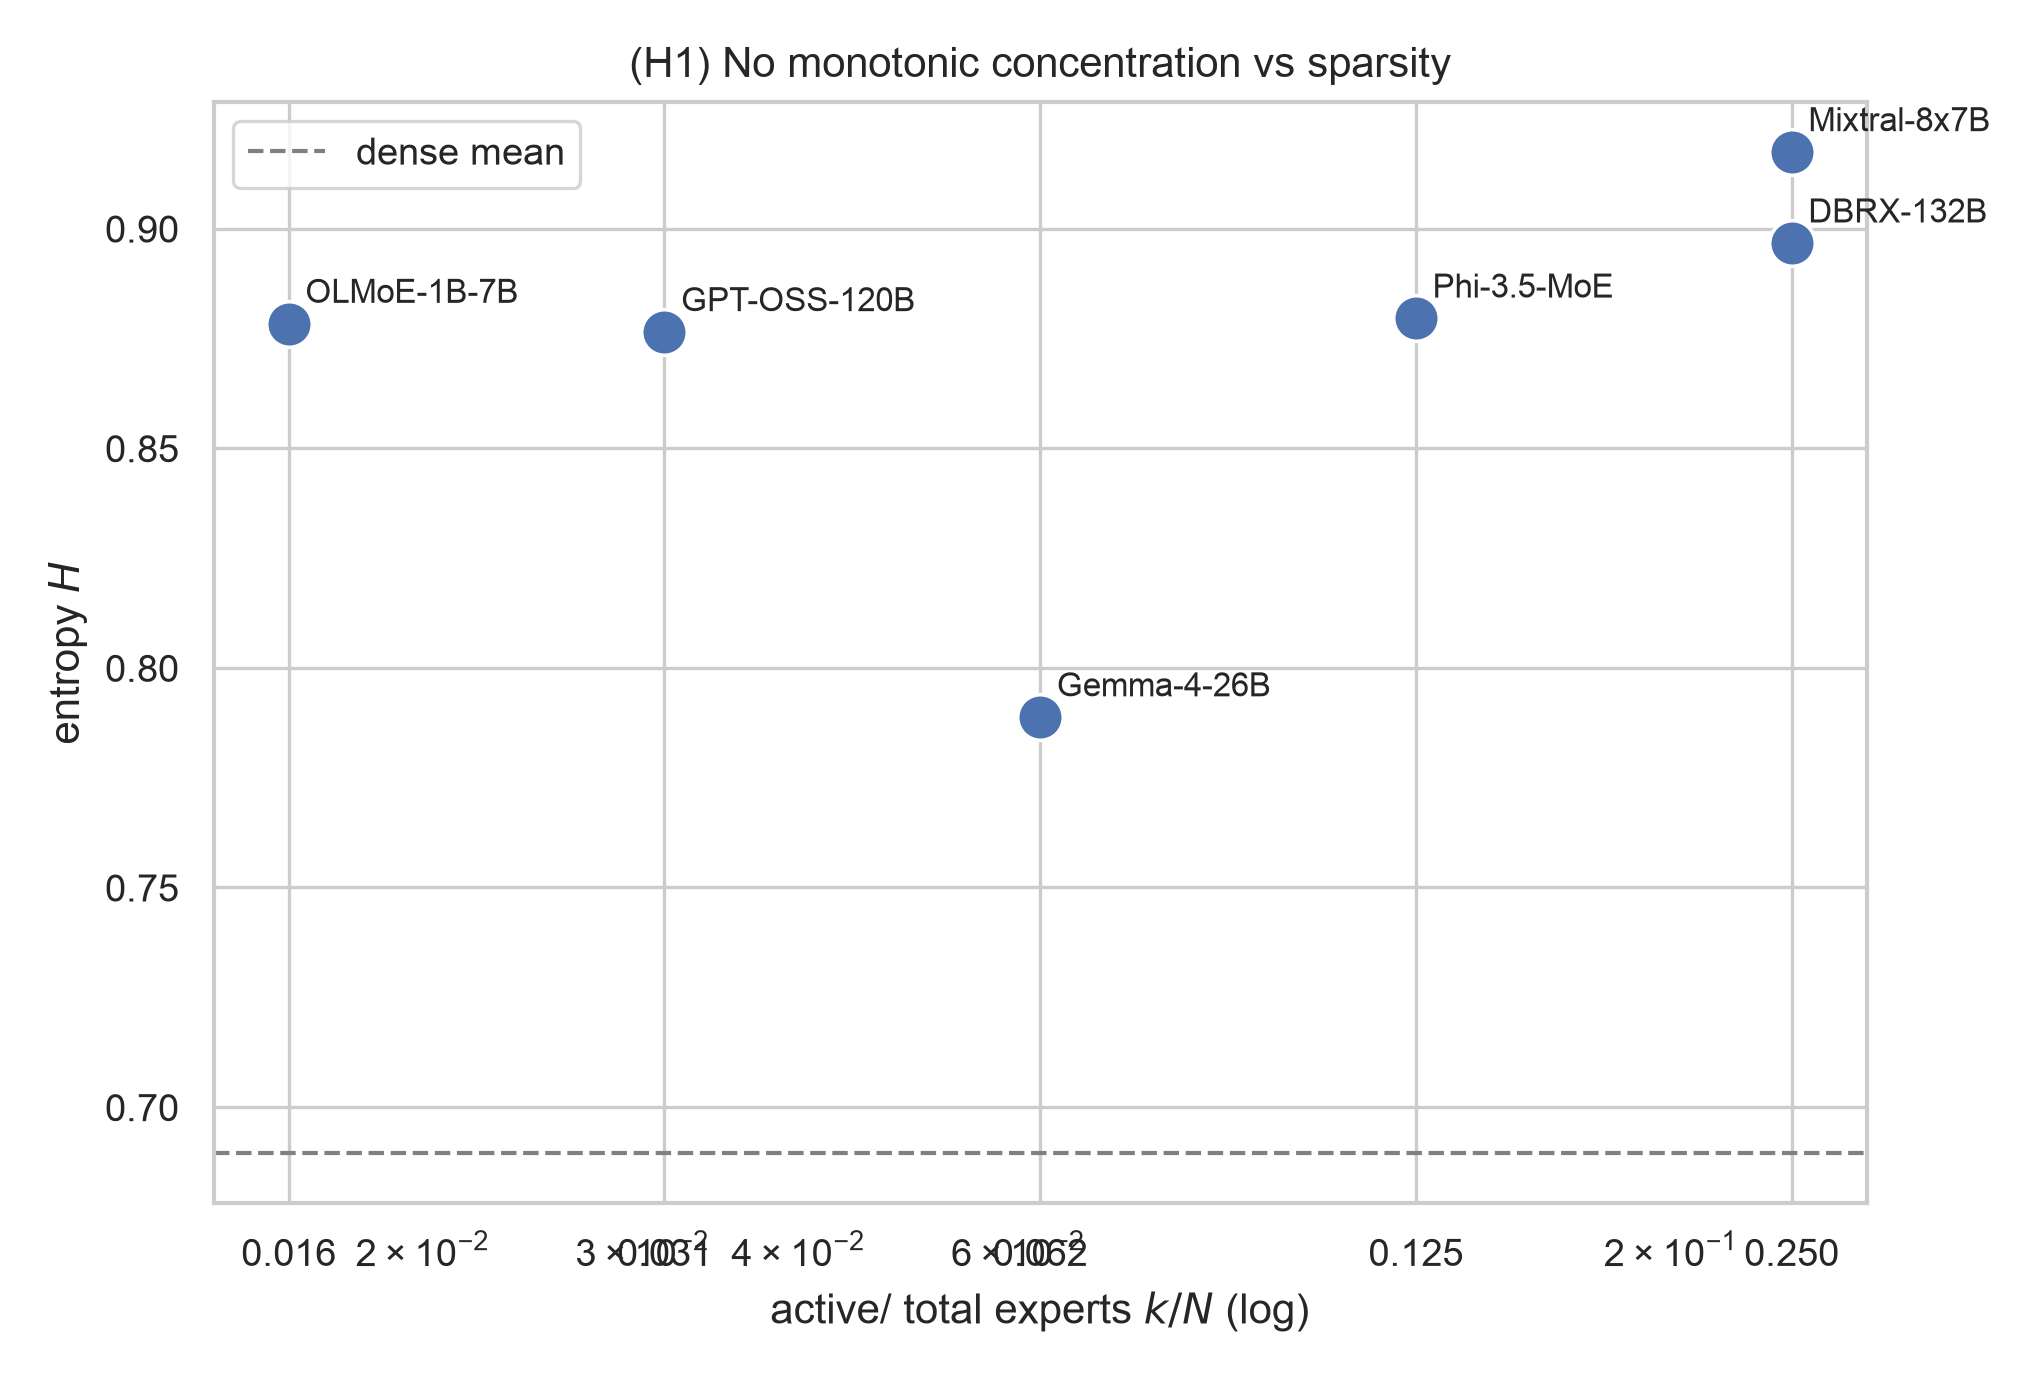
\includegraphics[width=\columnwidth]{fig3_h1_scatter.png}
\caption{Entropy vs.\ active fraction $k/N$ (log scale): H1 (sparser
$\Rightarrow$ more concentrated) is not supported ($\rho = 0.2$,
$p = 0.63$).}
\label{fig:scatter}
\end{figure}

\subsection{Top-fraction: no expert-level concentration}
Figure~\ref{fig:topfrac}: the top-5 experts hold only $2$--$11\%$ of
attribution mass across \emph{all} MoE rungs, and the top-$10\%$ share sits
at $0.35$--$0.66$. There is no small, stable ``fixable'' expert set.

\begin{figure}[t]
\centering
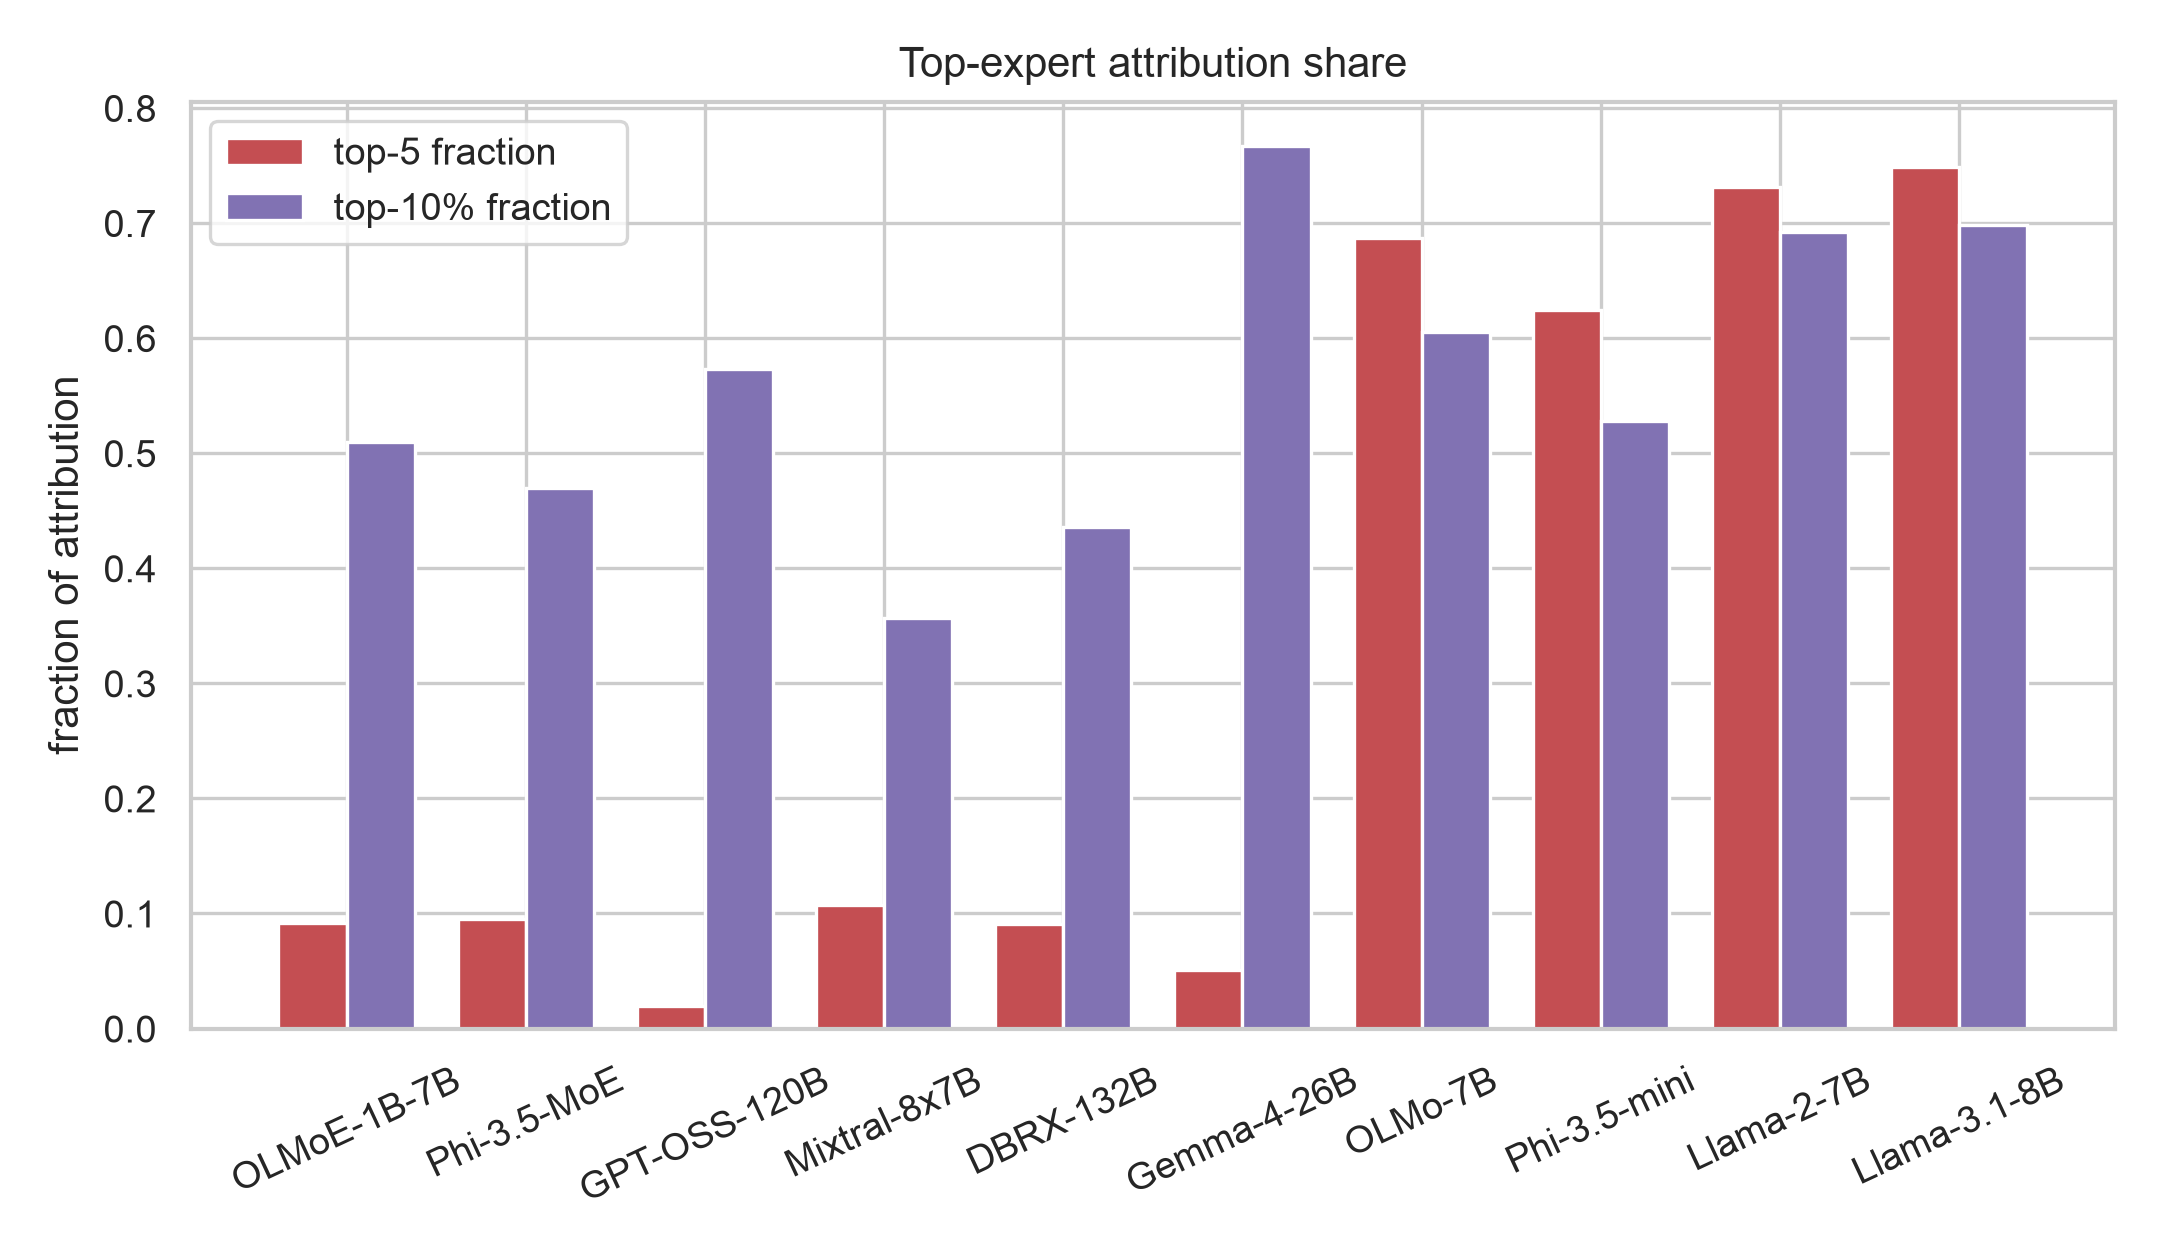
\includegraphics[width=\columnwidth]{fig4_top_fraction.png}
\caption{Top-5 and top-10\% share across the ladder.}
\label{fig:topfrac}
\end{figure}

\subsection{Dense vs.\ MoE: a real split, not a ladder}
Dense baselines ($H$: $0.630$--$0.758$; mean $0.689$, Table~\ref{tab:dense})
cluster clearly below every MoE rung ($0.822$--$0.919$). The separation
survives removal of the flagged models and is the robust signal of the
study---but it is a pointer-geometry effect: a dense layer is a single
aggregated player, which mechanically narrows the attribution distribution.
It does not validate bias concentration by the router.

\begin{figure}[t]
\centering
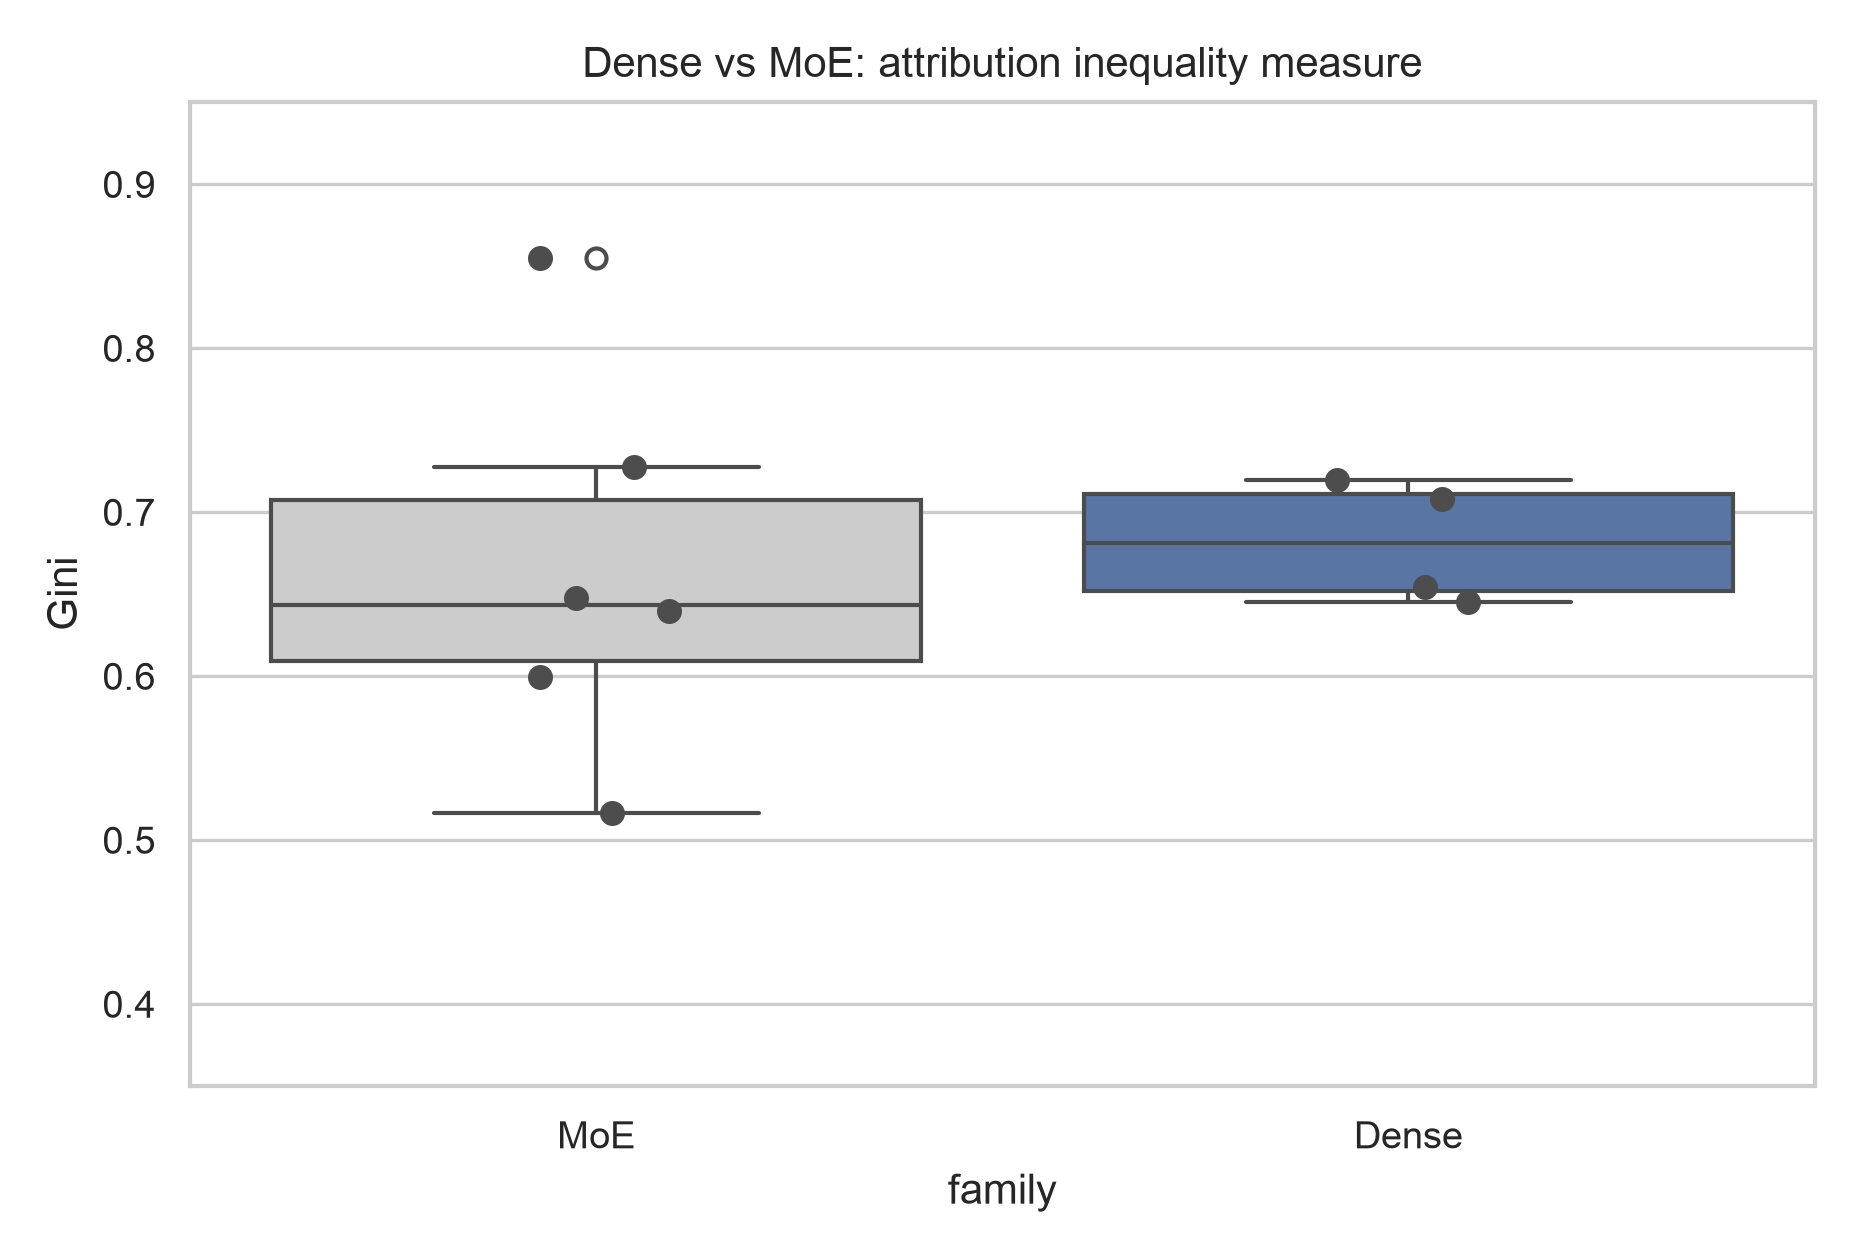
\includegraphics[width=\columnwidth]{fig5_dense_vs_moe.png}
\caption{Dense vs.\ MoE Gini.}
\label{fig:dense}
\end{figure}

\section{Robustness and Sensitivity}
\label{sec:robust}
\subsection{Run-to-run drift (v0 vs.\ v1)}
For the four models captured twice (OLMoE, Phi-3.5-MoE, Mixtral, DBRX; v0
with 400 pairs, v1 with 5000), the v0--v1 rerun drift floors are
$\mathrm{floor}_H = 0.022$ and $\mathrm{floor}_G = 0.047$ (max absolute
drift; mean absolute drift $0.014$ and $0.030$ respectively). Per-model
drift: OLMoE $\Delta H = -0.022$, $\Delta G = +0.047$; Phi-3.5-MoE
$\Delta H = -0.011$, $\Delta G = +0.027$; Mixtral $\Delta H = -0.0003$,
$\Delta G = +0.003$; DBRX $\Delta H = -0.022$, $\Delta G = +0.046$.
Pairwise ladder differences smaller than these floors (or than $2\times$ the
floor for cross-model comparisons, which carry error on both sides) are
classified as \emph{empirically unresolved}; the dense-vs-MoE entropy gap
($\ge 0.064$) exceeds the floor by $3$--$6\times$ and is the only robust
contrast. Split-half shards (two sets of 2500 pairs) for Mixtral/DBRX agree
to $\le 0.004$ in entropy.

\subsection{Permutation / null analysis}
We add (i) an expert-index permutation null that re-shuffles expert
identities within each run, and (ii) a reported-label permutation null
(paper-as-reported; per-prompt assignment not yet shipped, flagged in
Section~\ref{sec:limits}). On the cohort study below, the index null has
mean $0.31$ (sd $0.03$; $p_{95} = 0.37$), and only $0.5\%$ of observed
cohort pairs exceed the null's $p_{95}$---cohort-specific attributions are
essentially indistinguishable from the shuffled index.

\subsection{Model-set sensitivity audit}
\label{sec:verdict}
We re-run the monotonicity verdict across every defensible subset of the
ladder (all values from \path{outputs/s03_h1_verdict.json}, v1 runs
where valid, v0 otherwise):
\begin{itemize}
\item 6 models (full ladder): $\rho_H = 0.52$, $p = 0.29$; $\rho_G = -0.75$, $p = 0.08$;
\item 5 models (without GPT-OSS): $\rho_H = 0.67$, $p = 0.22$; $\rho_G = -0.87$, $p = 0.054$;
\item 5 models (paper ladder, without Gemma): $\rho_H = 0.67$, $p = 0.22$; $\rho_G = -0.87$, $p = 0.054$;
\item 4 models (without GPT-OSS and Gemma): $\rho_H = 0.74$, $p = 0.26$; $\rho_G = -0.95$, $p = 0.052$;
\item 3 distinct-sparsity rungs: $\rho_H = 0.50$, $p = 0.67$; $\rho_G = -1.00$ on 3 points.
\end{itemize}
No entropy statistic is significant at $p < 0.05$ in \emph{any} subset;
Gini never drops below $p = 0.05$ either except for the knife-edge
three-point case. The larger $|\rho_G|$ values are carried by the two
flagged endpoints (GPT-OSS $G = 0.724$, Gemma $G = 0.821$) and by
same-sparsity ties; drift-aware inspection shows most wrong-direction pairs
fall inside the empirical floors. The directional signal is therefore
fragile, subset-dependent, and not statistically supported---consistent
with the primary result $\rho = 0.2$, $p = 0.63$.

\subsection{Statistical method note}
The target procedure is a per-pair block bootstrap (resample pairs with
replacement, seed 42, $95\%$ percentile intervals) over the batch design;
flights are queued for most models, and \texttt{s04\_bootstrap\_cis.json}
reports MISSING for every model locally (per-pair $\phi$ payloads not synced
from the cluster). Consequently, no confidence-interval columns appear in
our tables; every concentration cell is a single measure and is flagged
\texttt{CI:pending} (Section~\ref{sec:limits}). The only landed bootstrap CI
at submission is the cohort JS mean, $95\%$ CI $[0.206, 0.231]$.

\subsection{Demographic-specificity}
Expanding on OLMoE with 85 demographically-defined cohorts, per-cohort
expert attributions versus the pooled distribution
(\path{exp5-demographic-specificity-olmoe-1b-7b-v1}) show a unimodal
Jensen--Shannon distance distribution with mean $0.22$ (sd $0.05$; bootstrap
$95\%$ CI $[0.206, 0.231]$), far below the expert-index permutation line
$0.31$ (Fig.~\ref{fig:js}); only $0.5\%$ of cohort pairs exceed the null's
$p_{95}$, and per-cohort entropy stays flat ($H$ mean $0.885$, sd $0.026$;
Gini mean $0.638$). No cohort is a ``specialist''---consistent with the
flat-ladder finding. The most divergent pairs (e.g.,
Vietnam$\times$software\_developer, JS $0.27$) do not form a coherent
demographic structure.

\begin{figure}[t]
\centering
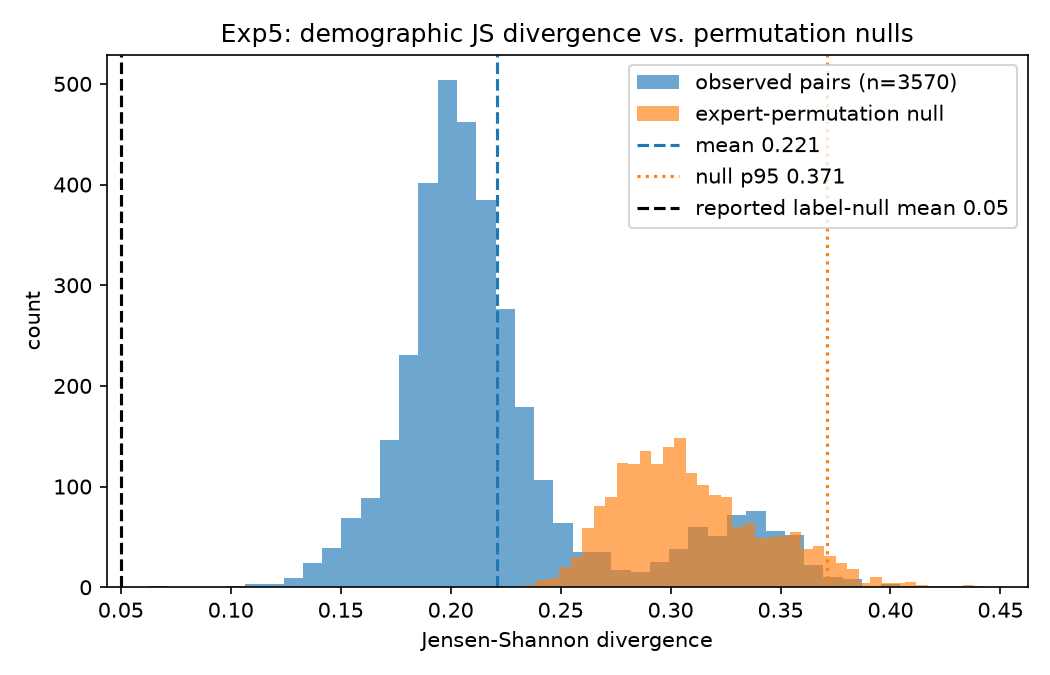
\includegraphics[width=\columnwidth]{s02_js_distribution.png}
\caption{JS distance between per-cohort and pooled expert attribution
distributions (OLMoE, 85 cohorts). The vertical line marks the
expert-index permutation null.}
\label{fig:js}
\end{figure}

\section{Discussion}
The honest picture: bias attributions are spread broadly and evenly across
the expert space in every MoE we could measure. Concentration claims are
not supported, and anything that looked like a trend traced to measurement
artifacts (an MXFP4-compromised run, a null-bias model, and v0/v1 drift) or
to tiny point clouds. The single robust separation is dense-per-layer vs.\
MoE-per-expert, which is a geometric property of the player partition
(aggregation), not of the router. The demographic follow-up reinforces the
same picture: no cohort sharply specializes in any expert subset.
Implication: ``prune the bias experts'' is not supported by this data;
interventions at the calibration or data level remain the defensible
options.

\section{Limitations and Uncertainty Flags}
\label{sec:limits}
\begin{itemize}
\item \textbf{GPT-OSS-120B (MXFP4) capture --- flag: \path{gpt-oss-pending}.}
Weights are 4-bit MXFP quantized; the fused multi-GPU forward crashes on
torch~2.6 + cu124 (\path{shared_memory_per_block_optin}). All figures
use the v0 bf16-dequantized single-GPU run (400 pairs, $H = 0.880$). The v1
directory holds all-zero $\phi$ (broken capture) and is \textbf{not cited}.
A clean rerun is queued; the GPT-OSS row in Table~\ref{tab:ladder} is
uncertainty-flagged until it lands.
\item \textbf{Per-pair bootstrap CIs --- flag: \texttt{CI:pending}.}
Bootstrap flights are queued for essentially all models; the DBRX per-pair
$\phi$ exists on the cluster but is not synced locally
(\path{s04_bootstrap_cis.json}: MISSING for all models). No CI columns
appear in any table; all concentration cells are single-measure. Only the
exp5 JS mean carries a CI ($[0.206, 0.231]$). An earlier draft quoted
bootstrap widths of $\pm 0.004$--$0.012$; those values are \emph{not}
reproducible from on-disk artifacts and are withdrawn here.
\item \textbf{Gemma-4-26B is a null-bias model --- flag:
\path{null-bias}.} Its mean bias gap $\approx 0$ and $47\%$ of its
$\phi$ are exactly zero; its concentration readings should be treated as
routing noise. Its $k/N$ uses the corrected $N_A = 240$ (an earlier
miscount of $960$ was fixed in \path{s03_h1_verdict.py}).
\item \textbf{Primary $\rho = 0.2$, $p = 0.63$ --- flag:
\path{small-n}.} With 3--6 ladder positions, Spearman power is limited
and $p$ thresholds are knife-edge; we therefore also report drift floors
and the explicit subset audit rather than a binary accept/reject.
\item \textbf{Label-permutation null --- flag: \allowbreak
\path{null:label-pending}.}
The reported-label null in \texttt{s02} was computed as-reported; the
per-prompt assignment is not yet shipped. The expert-index null used here
is on-disk and reproducible.
\item \textbf{Top-$k$ plumbing --- flag: \path{hooks:pending}.} $k$
(active experts) is read from router attributes at runtime
(\path{hooks.py}); DBRX's $N_A$ and any future config divergence may
alter $k/N$ assignment.
\end{itemize}

\section{Conclusion}
H1 is not supported: across six MoE models and four dense baselines with a
common attribution kernel, concentration metrics are flat and high
(normalized entropy $0.82$--$0.92$; top-5 share $2$--$11\%$), and no
monotonic sparsity-to-concentration trend survives drift, permutation, or
model-set audits ($\rho = 0.2$, $p = 0.63$ in the primary analysis). The
robust signals are the dense-vs-MoE offset (a player-partition geometry
effect) and the absence of demographic specialist structure. Expert-level
pruning of social bias is not supported as a strategy by this data.

\section*{Data \& Code}
\begin{itemize}\setlength\itemsep{0pt}
\item Runs and per-pair Shapley payloads:
  \path{expt-bias-1/results/*/result.json}.
\item Analysis scripts: \path{paper_figures_seaborn.py},
  \path{s01_exp1_stability.py}, \path{s02_exp5_js.py},
  \path{s03_h1_verdict.py}, \path{s04_bootstrap_cis.py}
  (all under \path{stats_analysis/scripts/}).
\item Outputs and figures: \path{stats_analysis/outputs/},
  \path{stats_analysis/figures/}.
\end{itemize}

\bibliographystyle{ACM-Reference-Format}
\begin{thebibliography}{99}
\bibitem{shapley1953} L.~S. Shapley. A Value for $n$-Person Games. In
  \emph{Contributions to the Theory of Games II}, Annals of Mathematics
  Studies 28, 1953.
\bibitem{lundberg2017} S.~M. Lundberg and S.-I.~Lee. A Unified Approach to
  Interpreting Model Predictions. In \emph{Advances in Neural Information
  Processing Systems (NeurIPS)}, 2017.
\bibitem{rozemberczki2022} B.~Rozemberczki, L.~Watson, P.~Bayer, H.-T.~Yang,
  O.~Kiss, S.~Nilsson, and R.~Sarkar. The Shapley Value in Machine
  Learning. \texttt{arXiv:2205.10702}, 2022.
\bibitem{shazeer2017} N.~Shazeer, A.~Mirhoseini, K.~Maziarz, A.~Davis,
  Q.~Le, G.~Hinton, and J.~Dean. Outrageously Large Neural Networks: The
  Sparsely-Gated Mixture-of-Experts Layer. In \emph{ICLR}, 2017.
\bibitem{lepikhin2021} D.~Lepikhin, H.~Lee, Y.~Xu, D.~Chen, O.~Firat,
  Y.~Huang, M.~Krikun, N.~Shazeer, and Z.~Chen. GShard: Scaling Giant
  Models with Conditional Computation and Automatic Sharding. In
  \emph{ICLR}, 2021.
\bibitem{fedus2022} W.~Fedus, B.~Zoph, and N.~Shazeer. Switch Transformers:
  Scaling to Trillion Parameter Models with Simple and Efficient Sparsity.
  \emph{Journal of Machine Learning Research}, 23(120):1--39, 2022.
\bibitem{jiang2024} A.~Q.~Jiang \emph{et al.} Mixtral of Experts.
  \texttt{arXiv:2401.04088}, 2024.
\bibitem{muennighoff2024} N.~Muennighoff \emph{et al.} OLMoE: Open
  Mixture-of-Experts Language Models. \texttt{arXiv:2409.12288}, 2024.
\bibitem{gemmaTeam2024} Gemma Team (Google). Gemma: Open Models Based on
  Gemini Research and Technology. \texttt{arXiv:2403.08295}, 2024.
\bibitem{cai2024} Z.~Cai \emph{et al.} A Survey on Mixture of Experts.
  \texttt{arXiv:2407.06204}, 2024.
\bibitem{nadeem2021} M.~Nadeem, A.~Bethke, and S.~Reddy. StereoSet: Measuring
  Stereotypical Bias in Pretrained Language Models. In \emph{ACL}, 2021.
\bibitem{parrish2022} A.~Parrish, A.~Chen, N.~Nangia, V.~Padmakumar,
  J.~Phang, J.~Thompson, P.~M.~Htut, and S.~R.~Bowman. BBQ: A
  Hand-Built Bias Benchmark for Question Answering. In \emph{Findings of
  ACL}, 2022.
\bibitem{liang2023} P.~Liang \emph{et al.} Holistic Evaluation of Language
  Models. \emph{Transactions of the Association for Computational
  Linguistics}, 11:1--48, 2023.
\bibitem{mehrabi2021} N.~Mehrabi, F.~Morstatter, N.~Saxena, K.~Lerman, and
  A.~Galstyan. A Survey on Bias and Fairness in Machine Learning. \emph{ACM
  Computing Surveys}, 54(6):1--35, 2021.
\bibitem{moe_research_2026} MoE-Bias-Research-Group. Routing-Shapley
  Bias-Concentration Study: Code and Artifacts (expt-bias-1), 2026.
\end{thebibliography}

\end{document}
